
\documentclass{beamer}

\usepackage{algpseudocode, color, colortbl, listings, multicol, MnSymbol, tikz}

\usepackage{hyperref}
\hypersetup{
    colorlinks=true,
    urlcolor=blue,
}

\usetheme{Montpellier}
\usecolortheme{rose}

\tikzset{treenode/.style={draw, circle, minimum size=8mm}}

% page numbers, from
% https://tex.stackexchange.com/questions/137022/how-to-insert-page-number-in-beamer-navigation-symbols
\expandafter\def\expandafter\insertshorttitle\expandafter{%
  \insertshorttitle\hfill%
  \insertframenumber\,/\,\inserttotalframenumber}

\definecolor{Gray}{gray}{0.8}
\newcolumntype{g}{>{\columncolor{Gray}}c}

\newcommand{\stanza}{ \\~\ }

\title{13. Dynamic Programming for Longest Common Subsequence and Optimal Binary Search Trees}
\subtitle{CPSC 535}
\author{Kevin A. Wortman}
\institute{ 
\includegraphics[height=2cm]{csuf-logo-cmyk} }
\date{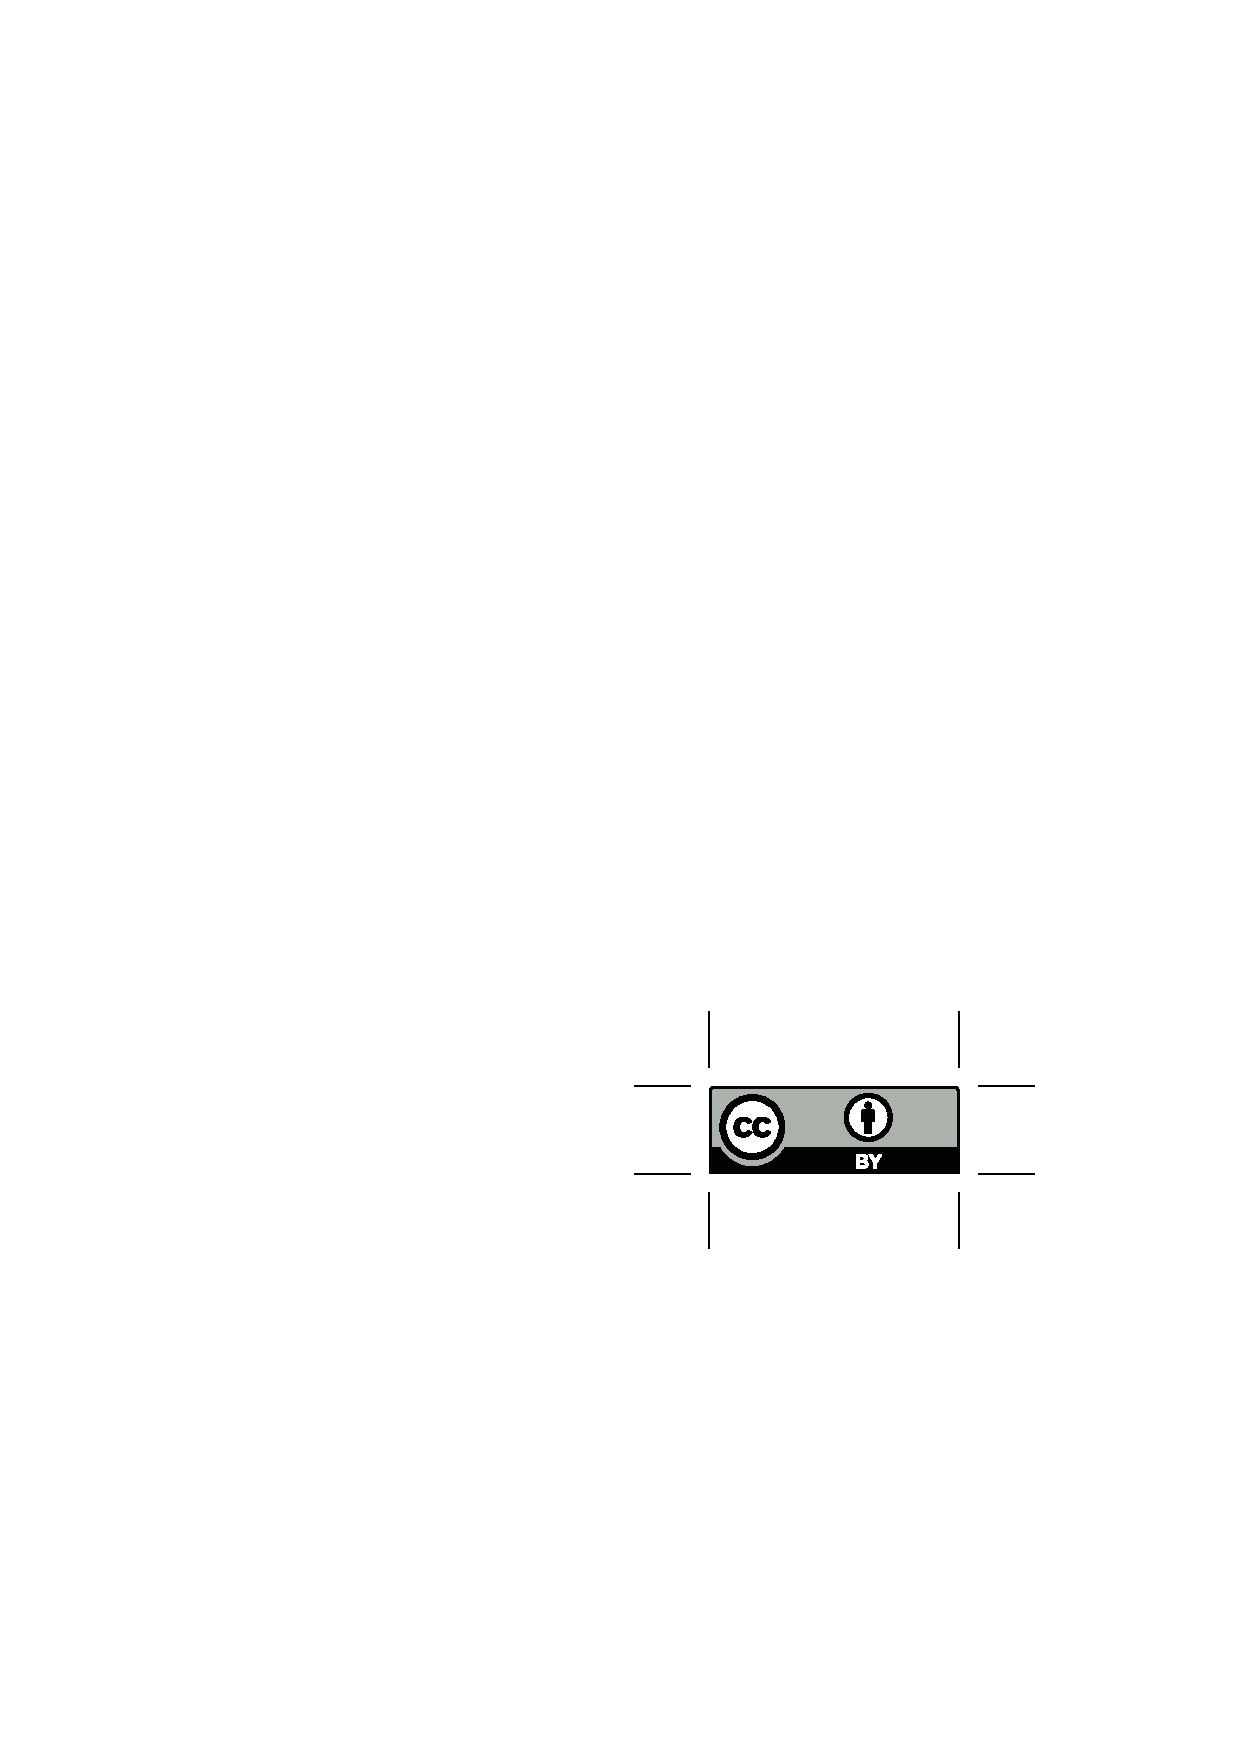
\includegraphics[height=14pt]{by} \\

{\tiny
This work is licensed under a
\href{http://creativecommons.org/licenses/by/4.0/}{Creative Commons Attribution 4.0 International License}.
}}

\begin{document}

\begin{frame}
  \titlepage
\end{frame}

\begin{frame} \frametitle{Big Idea: Alternative Kinds of Solutions}
  \begin{itemize}
  \item So far
    \begin{itemize}
      \item Step 2. Derive a \textbf{recurrence} for an optimal value.
      \item Recall rod cutting:
        \[ r_i = \max_{1 \leq i \leq n} (p_i + r_{n-i}) \]
      \item Recall matrix chain multiplication:
        \[ r_{i, j} = \min_{i \leq k \leq \, j} r_{i, k} + r_{k+1, \, j} + p_{i-1} p_k p_j \]
    \end{itemize}
  \item Now: longest common subsequence (LCS)
    \begin{itemize}
      \item not simply minimizing/maximizing one expression
      \item instead, choose between \textbf{three alternatives}
      \item \textbf{2D table}, like matrix chain
    \end{itemize}
  \end{itemize}
\end{frame}

\begin{frame} \frametitle{Subsequences}
  \begin{itemize}
  \item Let $X=\langle x_1, x_2, \ldots, x_m \rangle$ and $Y=\langle y_1, y_2, \ldots, y_n \rangle$ be two sequences
  \item Define \textbf{prefix} notation: $X_k = \langle x_1, \ldots, x_k \rangle; X_0 = \langle \rangle$
  \begin{itemize}
    \item if $X=\langle 2, 7, 8, 1, 7, 1, 2 \rangle$ then $X_3 = \langle 2, 7, 8 \rangle $
  \end{itemize}
  \item Informally: a \textbf{subsequence} of $Y$ is a copy of $Y$ with some elements removed
  \item Formally: $X$ is a \textbf{subsequence} of $Y$ if there exists an increasing sequence of indices $\langle i_1, i_2, \ldots, i_k \rangle$ such that, for all $j \in [1, k], x_j = y_{i_j}$
  \item Example: for $X=\langle B, C, D, B\rangle$ and $Y=\langle A, B, C, B, D, A, B \rangle,$ $X$ is a subsequence of $Y$ with index sequence $\langle 2, 3, 5, 7 \rangle$
  \end{itemize}
\end{frame}

\begin{frame} \frametitle{Common Subsequence}
  \begin{itemize}
  \item $Z$ is a \textbf{common subsequence} of $X$ and $Y,$ if $Z$ is a subsequence $X$ and $Z$ is a subsequence of $Y$
  \item a \textbf{longest common subsequence} is a common subsequence of maximum length
  \item Example: let $X=\langle A, B, C, B, D, A, B \rangle $  and $Y=\langle B, D, C, A, B, A \rangle$ 
  \item $Z=\langle B, C, A \rangle$ is a common subsequence
  \item $Z=\langle B, C, B, A \rangle$ is a longest common subsequence
  \end{itemize}
\end{frame}

\begin{frame} \frametitle{Longest Common Subsequence}

  \emph{Longest Common Subsequence (LCS) solution problem} \\
  \textbf{input:} sequences $X=\langle x_1, x_2, \ldots, x_m \rangle$ and $Y=\langle y_1, y_2, \ldots, y_n \rangle$
  \textbf{output:} a longest common subsequence of $X$ and $Y$ \stanza
  
  \emph{Longest Common Subsequence (LCS) value problem} \\
  \textbf{input:} (same) \\
  \textbf{output:} the length of a longest common subsequence of $X$ and $Y$ \stanza

\end{frame}

\begin{frame} \frametitle{Design Process}
  \begin{enumerate}
    \item Identify the problem's \textbf{solution} and \textbf{value}, and note which is our \textbf{goal}.
    \item Derive a \textbf{recurrence} for an optimal value.
    \item Design a divide-and-conquer algorithm that computes an \textbf{optimal value}.
    \item Design a dynamic programming algorithm that computes an \textbf{optimal value}.
    \begin{enumerate}
      \item \textbf{top-down} alternative: add table base case (\textbf{memoization})
      \item \textbf{bottom-up} alternative: rewrite to use bottom-up loops instead of recursion
    \end{enumerate}
    \item (if goal is a solution algo.) Design a dynamic programming algorithm that computes an \textbf{optimal solution}.
  \end{enumerate}
  \end{frame}

  \begin{frame} \frametitle{Longest Common Subsequence Step 1}
    \begin{enumerate}
      \item Identify the problem's \textbf{solution} and \textbf{value}, and note which is our \textbf{goal}.
      \stanza
    \end{enumerate}

    \begin{itemize}
      \item \textbf{solution:} a sequence e.g. $\langle B, C, B, A \rangle$
      \item \textbf{value:} integer length of a sequence e.g. 4
      \item eventual goal is solution
      \item start with value
    \end{itemize}
  \end{frame}
  
  \begin{frame} \frametitle{Longest Common Subsequence Step 2}
    \begin{enumerate}
      \setcounter{enumi}{1}
      \item Derive a \textbf{recurrence} for an optimal value.
      \stanza
    \end{enumerate}
    \begin{itemize}
      \item Recall input: $X=\langle x_1, x_2, \ldots, x_m \rangle$ and $Y=\langle y_1, y_2, \ldots, y_n \rangle$
      \item Recall \emph{prefix:} $X_i$ is first $i$ elements of $X$
      \item Define $LCS(X, Y) \equiv$ length of longest common subsequence of $X$ and $Y$
      \item We need to define $LCS$ recursively
      \end{itemize}

      \end{frame}
      \begin{frame} \frametitle{Longest Common Subsequence Step 2}
        \begin{enumerate}
          \setcounter{enumi}{1}
          \item Derive a \textbf{recurrence} for an optimal value.
          \stanza
        \end{enumerate}
        \begin{itemize}
          \item \textbf{Idea:} If last symbols $x_m=y_n$ match, then extend a shorter common subsequence:
            $LCS(X, Y) = LCS(X_{m-1}, Y_{n-1}) + 1$
          \item Else ($x_m \ne y_n$), have to omit $x_m$ or $y_n$
            \begin{itemize}
            \item Omit $x_m$: $LCS(X, Y) = LCS(X_{m-1}, Y)$
            \item Omit $y_n$: $LCS(X, Y) = LCS(X, Y_{n-1})$
            \item Want \textbf{longest} so 
            \[ LCS(X, Y) = \max(LCS(X_{m-1}, Y), LCS(X, Y_{n-1})) \]
              \end{itemize}
          \end{itemize}
    \end{frame}

    \begin{frame} \frametitle{Example}
      \begin{itemize}
        \item Suppose $X=\langle A, B, A, D \rangle$ and $Y = \langle B, B, A, C, D \rangle$
        \item Last symbols match,  $x_4=y_5=D,$ so
          \begin{align*}
            LCS(X,Y) &= LCS(X_{m-1}, Y_{n-1}) + 1 \\
            &= LCS(\langle A, B, A \rangle, \langle B, B, A, C \rangle) + 1
          \end{align*}
        \item Now suppose $X=\langle A, B, A, D \rangle$ and $Y = \langle B, B, A, C, C \rangle$
        \item Last symbols differ ($x_4=D$ but $y_5=C$), so
          {\footnotesize
          \begin{align*}
            LCS(X,Y)
            &= \max(LCS(X_{m-1}, Y_n), LCS(X_m, Y_{n-1})) \\
            &= \max(\langle A, B, A \rangle, \langle B, B, A, C, C \rangle), LCS(\langle A, B, A, D \rangle, \langle B, B, A, C \rangle)) 
          \end{align*}
          }
        \end{itemize}
        
    \end{frame}
    
  \begin{frame} \frametitle{Longest Common Subsequence Step 2}
    \begin{enumerate}
      \setcounter{enumi}{1}
      \item Derive a \textbf{recurrence} for an optimal value.
      \stanza
    \end{enumerate}

\[ LCS(X_m, Y_n) =
    \begin{cases}
      0 & m=0 \\
      0 & n=0 \\
      LCS(X_{m-1}, Y_{n-1}) + 1 & x_m=x_n \\
      \max(LCS(X_{m-1}, Y_n), LCS(X_m, Y_{n-1})) & \text{otherwise}
    \end{cases}
  \]
  \end{frame}

\begin{frame} \frametitle{Longest Common Subsequence Step 3}
  \begin{enumerate}
    \setcounter{enumi}{2}
    \item Design a divide-and-conquer algorithm that computes an \textbf{optimal value}.
    \stanza
  \end{enumerate}

  {\scriptsize
  \begin{algorithmic}[1]
    \Function{LCS-DC}{$X[1..m], Y[1..n]$}
    \If{ $m==0$ or $n==0$ }
      \State \Return{ 0 }
    \ElsIf{ $X[m] == Y[n]$ }
      \State \Return{ $\text{LCS-DC}(X[1..m-1], Y[1..n-1]) + 1$ }
    \Else
      \State \Return{ $\max(\text{LCS-DC}(X[1..m-1], Y[1..n]), \text{LCS-DC}(X[1..m], Y[1..n-1])$ }
    \EndIf
    \EndFunction
  \end{algorithmic}
  }
\end{frame}
    
  \begin{frame} \frametitle{Matrix Chain Multiplication Step 4.a}
    \begin{enumerate}
      \setcounter{enumi}{3}
      \item Design a dynamic programming algorithm that computes an \textbf{optimal value}.
      \begin{enumerate}
        \item \textbf{top-down} alternative: add table base case (\textbf{memoization})
        \stanza
      \end{enumerate}
  \end{enumerate}

  \begin{itemize}
    \item Recall \textbf{memoization:} use a hash dictionary to make a ``memo'' of pre-calculated solutions
    \item create hash table $T$
    \item use pair $(m, n)$ as key in table $T,$ storing $LCS(X_m, Y_n)$
  \end{itemize}
  
\end{frame}  

\begin{frame} \frametitle{Matrix Chain Multiplication Step 4.a}
  {\scriptsize
  \begin{algorithmic}[1]
    \Function{LCS-MEMOIZED}{$X[1..m], Y[1..n]$}
    \State HASH-TABLE-CREATE($T$)
    \State \Return{LCS-M($T, X, Y$)}
    \EndFunction
    \Function{LCS-M}{$T, X[1..m], Y[1..n]$}
    \State $q = $ HASH-TABLE-SEARCH($T, (m, n)$)
    \If{ $q \ne$ NIL }
      \State \Return{ $q$ }
    \EndIf
    \If{ $m==0$ or $n==0$ }
      \State $q=0$
    \ElsIf{ $X[m] == Y[n]$ }
      \State $q = \text{LCS-M}(T, X[1..m-1], Y[1..m-1]) + 1$
    \Else
      \State $q = \max(\text{LCS-M}(X[1..m-1], Y[1..n]), \text{LCS-M}(X[1..m], Y[1..n-1])$
    \EndIf
    \State $q.key = (m, n)$
    \State HASH-TABLE-INSERT($q$)
    \State \Return{$q$}
    \EndFunction
  \end{algorithmic}
  }
\end{frame}

\begin{frame} \frametitle{Memoized Algorithm Analysis}
  \begin{itemize}
    \item $T$ contains $\Theta(n^2)$ pairs $(m, n)$
    \item each entry is inserted exactly once
    \item in the general case, LCS-M takes $\Theta(1)$ expected time
    \item $\Rightarrow$ LCS-MEMOIZED takes $\Theta(n^2)$ expected time
  \end{itemize}
\end{frame}

\begin{frame} \frametitle{Longest Common Subsequence Step 4.b}
  \begin{enumerate}
    \setcounter{enumi}{3}
    \item Design a dynamic programming algorithm that computes an \textbf{optimal value}.
    \begin{enumerate}
      \item \textbf{top-down} alternative: add table base case (\textbf{memoization})
      \item \textbf{bottom-up} alternative: rewrite to use bottom-up loops instead of recursion
      \stanza
    \end{enumerate}
\end{enumerate}

\begin{itemize}
  \item create 2D array $c$ where $c[i][\, j] = LCS(X_i, Y_j)$
  \item \textbf{bottom-up:} write an explicit \textbf{for} loop that computes and stores every general case
  \item need to order loops so we never use an uninitialized element
  \item $\therefore$ initialize all base cases before any general case
\end{itemize}
\end{frame}
  
\begin{frame} \frametitle{Longest Common Subsequence Step 4.b}
  {\footnotesize
  \begin{algorithmic}[1]
    \Function{LCS-BU}{$X[1..m], Y[1..n]$}
    \State Create array $c[0..m][0..n]$ \Comment{unusual index range}
    \For{$i$ from 0 to $m$}
      \State $c[i][0] = 0$
    \EndFor
    \For{$j$ from 1 to $n$} \Comment{only initialize $c[0][0]$ once}
      \State $c[0][j] = 0$
    \EndFor
    \For{$i$ from 1 to $m$}
      \For{$j$ from $1$ to $n$}
        \If{ $X[i]==Y[j]$ }
          \State $c[i][j] = c[i-1][j-1] + 1$
        \Else
          \State $c[i][j] = \max(c[i-1][j], c[i][j-1])$
        \EndIf
      \EndFor
    \EndFor
    \State \Return $c[m][n]$
    \EndFunction
  \end{algorithmic}
  }
\end{frame}

\begin{frame} \frametitle{Bottom-Up Analysis}
  \begin{itemize}
    \item LCS-BU is clearly $\Theta(n^2)$ time
    \item (easy analysis)
  \end{itemize}
\end{frame}

\begin{frame} \frametitle{Longest Common Subsequence Step 5}
  \begin{enumerate}
    \setcounter{enumi}{4}
    \item (if goal is a solution algo.) Design a dynamic programming algorithm that computes an \textbf{optimal solution}.
    \stanza
  \end{enumerate}

  \begin{itemize}
    \item \textbf{idea:} for each $(i, j),$ record which alternative sub-solution defines $c[i][\, j]:$
      \begin{itemize}
        \item $\nwarrow \equiv c[i-1][\, j-1]$
        \item $\uparrow \equiv c[i-1][\, j]$
        \item $\leftarrow \equiv c[i][\, j - 1]$
      \end{itemize}
    \item define
      \[ b[i][\, j] \in \{ \nwarrow, \uparrow, \leftarrow \} \]
    \item rewrite $\max(c[i-1][j], c[i][j-1])$ as \textbf{if}/\textbf{else} so we can update $b[i][\, j]$
  \end{itemize}
\end{frame}

\begin{frame} \frametitle{Longest Common Subsequence Step 5}
  {\tiny
  \begin{algorithmic}[1]
    \Function{LCS-SOLUTION}{$X[1..m], Y[1..n]$}
    \State Create arrays $c[0..m][0..n]$ and $b[1..m][1..n]$ \Comment{different index ranges}
    \For{$i$ from 0 to $m$}
      \State $c[i][0] = 0$
    \EndFor
    \For{$j$ from 1 to $n$} \Comment{only initialize $c[0][0]$ once}
      \State $c[0][j] = 0$
    \EndFor
    \For{$i$ from 1 to $m$}
      \For{$j$ from $1$ to $n$}
        \If{ $X[i]==Y[j]$ }
          \State $c[i][j] = c[i-1][\, j-1] + 1$
          \State $b[i][j] = \nwarrow$
        \ElsIf{ $c[i-1][j] \geq c[i][\, j-1]$ }
          \State $c[i][j] = c[i-1][\, j]$
          \State $b[i][j] = \uparrow$
        \Else
        \State $c[i][j] = c[i][\, j-1]$
        \State $b[i][j] = \leftarrow$
      \EndIf
      \EndFor
    \EndFor
    \State \Return $\text{LCS-BTRACK}(b, X, m, n)$
    \EndFunction
  \end{algorithmic}
  }
\end{frame}

\begin{frame} \frametitle{Longest Common Subsequence Step 5}
  {\small
  \begin{algorithmic}[1]
    \Function{LCS-BTRACK}{$b[1..m][1..n], X[1..m], i, j$}
    \If{ $i==0$ or $j==0$ }
      \State \Return{$\langle \rangle$} \Comment{empty sequence}
    \EndIf
    \If{ $b[i][j]==\nwarrow$ }
      \State \Return{$\text{LCS-BTRACK}(b, X, i-1, j-1) + \langle X[i] \rangle$} \Comment{append}
    \ElsIf{ $b[i][j]==\uparrow$ }
      \State \Return{$\text{LCS-BTRACK}(b, X, i-1, j)$}
    \Else
      \State \Return{$\text{LCS-BTRACK}(b, X, i, j-1)$}
    \EndIf
    \EndFunction
  \end{algorithmic}
  }
\end{frame}

\begin{frame} \frametitle{Review: Binary Search Trees}
\begin{itemize}
  \item Recall \textbf{Binary Search Tree (BST):} fundamental data structure
  \item \textbf{Depth} of node $x$ = length of path from root to $x$
  \item \textbf{Height} of tree = maximum depth of any node
  \item Time of a search = \textbf{depth} of search path
  \item Height
    \begin{itemize}
      \item worst case $= \Theta(n)$
      \item best case $= \Theta(\log n)$
    \end{itemize}
  \item self-balancing BST maintains $\Theta(\log n)$ height
  \end{itemize}
\end{frame}

\begin{frame} \frametitle{Worst-Case BSTs}
  \begin{center}
    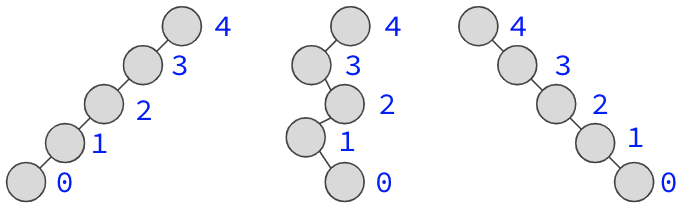
\includegraphics[height=1.3in]{bst_worst_case.png}
  \end{center}
\end{frame}

\begin{frame} \frametitle{Best-Case BST}
  \begin{center}
    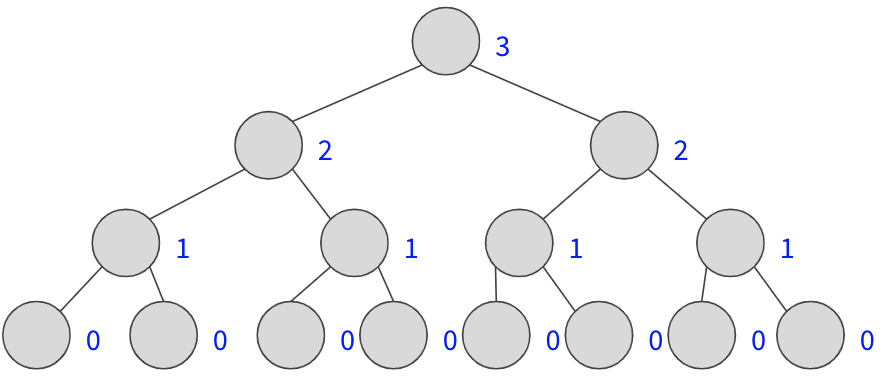
\includegraphics[height=1.5in]{bst_balanced.png}
  \end{center}
\end{frame}

\begin{frame} \frametitle{Optimal BSTs}
  \begin{itemize}
    \item Fix the sequence of search operations
    \item \textbf{Optimal} BST: minimizes total search time
      \begin{itemize}
        \item including constant factors
      \end{itemize}
    \item Total time for $n$ elements and $k$ searches:
      \begin{itemize}
        \item any self-balancing BST: $O(k \log n)$
        \item optimal BST: $O(k \log n)$ with lowest possible constant factor
      \end{itemize}
    \item Goal
      \begin{itemize}
        \item frequencly-visited elements near root
        \item rarely-visited elements near leaves
        \item tricky because a path visits multiple nodes; all count
      \end{itemize}
  \end{itemize}
\end{frame}

\begin{frame} \frametitle{Problem Setup}
\begin{itemize}
  \item Given:
    \begin{itemize}
      \item ordered keys $K = \langle k_1, k_2, \ldots, k_n \rangle$
      \item ``dummy'' values $d_0, d_1, \ldots, d_n$ represent values of failed searches, between keys
    \end{itemize}
  \item for a given search and index $i$,
  \begin{itemize}
    \item $p_i = $ probability that this is a successfull search for $k_i$
    \item $q_i = $ probability that this is a failed search for value $d_i$
  \end{itemize}
\end{itemize}
\end{frame}

\begin{frame} \frametitle{Problem Setup}
\begin{center}
  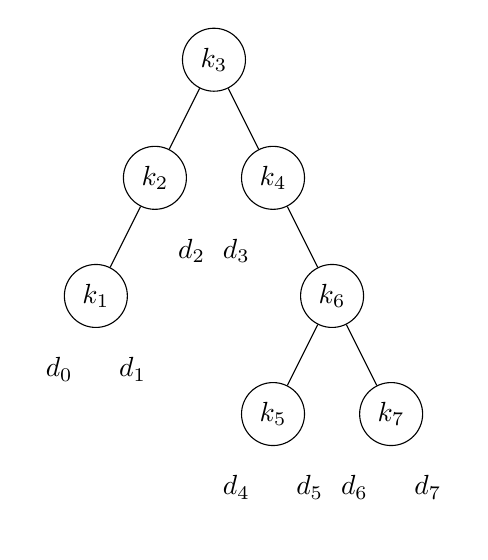
\begin{tikzpicture}[
      every node/.style={treenode}
    ]
    \node (root) {$k_3$}
    child { node {$k_2$}
        child { node {$k_1$}
          child { edge from parent [draw=none] node[draw=none] {$d_0$} }  
          child { edge from parent [draw=none] node[draw=none] {$d_1$} }
        }
        %child[missing] { node {} }
        child { edge from parent [draw=none] node[draw=none] {$d_2$} }
    }
    child { node {$k_4$}
    child { edge from parent [draw=none] node[draw=none] {$d_3$} }
        child { node {$k_6$}
            child { node {$k_5$}
              child { edge from parent [draw=none] node[draw=none] {$d_4$} }
              child { edge from parent [draw=none] node[draw=none] {$d_5$} }
            }
            child { node {$k_7$}
              child { edge from parent [draw=none] node[draw=none] {$d_6$} }
              child { edge from parent [draw=none] node[draw=none] {$d_7$} }
          }
        }
    };
  \end{tikzpicture}
\end{center}
\end{frame}

\begin{frame} \frametitle{Expected Search Cost}
  Every search ends in a key $k_i$ or dummy $d_i,$ so
    \[ \sum_{i=1}^n p_i + \sum_{i=0}^n q_i = 1. \]

  For tree $T,$
  \begin{align*}
    E[\text{search in} T] & = \sum_{i=1}^n (\text{depth}_T(k_i)+1) \cdot p_i + \sum_{i=0}^n (\text{depth}_T(d_i)) \cdot q_i \\
      & = 1 + \sum_{i=1}^n (\text{depth}_T(k_i)) \cdot p_i + \sum_{i=0}^n (\text{depth}_T(d_i)) \cdot q_i \\
  \end{align*}
  Have: probabilities $p_1, \ldots, p_n$ and $q_0, \ldots, q_n$ \\
  Need: shape $T$ to minimize sum
\end{frame}
  
\begin{frame} \frametitle{Optimal BST Problem}

  \emph{Optimal Binary Search Tree (BST) solution problem} \\
  \textbf{input:} keys $K=\langle k_1, k_2, \ldots, k_n \rangle;$ successfull-search probabilities $p_1, p_2, \ldots, p_n;$ and failed-search probabilities $q_0, q_1, \ldots, q_n$ \\  
  \textbf{output:} a BST $T$ that contains $K$ with minimum expected search cost  \stanza
  
  \emph{Optimal Binary Search Tree (BST) value problem} \\
  \textbf{input:} successfull-search probabilities $p_1, p_2, \ldots, p_n;$ and failed-search probabilities $q_0, q_1, \ldots, q_n$ \\  
  \textbf{output:} the minimum expected search cost of a tree that contains $K$ \stanza

  (Note: keys $K$ unneeded for value problem.)
\end{frame}

\begin{frame} \frametitle{Design Process}
  \begin{enumerate}
    \item Identify the problem's \textbf{solution} and \textbf{value}, and note which is our \textbf{goal}.
    \item Derive a \textbf{recurrence} for an optimal value.
    \item Design a divide-and-conquer algorithm that computes an \textbf{optimal value}.
    \item Design a dynamic programming algorithm that computes an \textbf{optimal value}.
    \begin{enumerate}
      \item \textbf{top-down} alternative: add table base case (\textbf{memoization})
      \item \textbf{bottom-up} alternative: rewrite to use bottom-up loops instead of recursion
    \end{enumerate}
    \item (if goal is a solution algo.) Design a dynamic programming algorithm that computes an \textbf{optimal solution}.
  \end{enumerate}
  \end{frame}

  \begin{frame} \frametitle{Optimal BST Step 1}
    \begin{enumerate}
      \item Identify the problem's \textbf{solution} and \textbf{value}, and note which is our \textbf{goal}.
      \stanza
    \end{enumerate}

    \begin{itemize}
      \item \textbf{solution:} a BST $T$
      \item \textbf{value:}
      $E[\text{search in} T] = 1 + \sum_{i=1}^n (\text{depth}_T(k_i)) \cdot p_i + \sum_{i=0}^n (\text{depth}_T(d_i)) \cdot q_i $
      \item goal is value
    \end{itemize}
  \end{frame}
  
\begin{frame} \frametitle{Optimal BST Step 2}
  \begin{enumerate}
    \setcounter{enumi}{1}
    \item Derive a \textbf{recurrence} for an optimal value.
    \stanza
  \end{enumerate}
  \begin{itemize}
    \item Make one decision and recurse for the rest
    \item Decision: \textbf{choose some key to be root}
    \item Define $e[i, j] = E[\text{search in optimal tree containing } k_i, \ldots, k_j ]$
    \item Denote empty tree with $j=i-1$
    \item Base case: empty tree; cost is $q_{i-1}$
    \item General case:
      \begin{itemize}
        \item choose a split index $r$
        \item recursively compute left subtree $e[i, r-1]$
        \item recursively compute right subtree $e[r+1, j]$
        \item add root on top; increases depths of subtrees
      \end{itemize}
  \end{itemize}
\end{frame}

\begin{frame} \frametitle{Optimal BST Step 2}
  \begin{itemize}
    \item Place root atop two subtrees
    \item +1 to path length of every descendant
    \item Recall
      \begin{align*}
        E[\text{search in} T] & = \sum_{i=1}^n (\text{depth}_T(k_i)+1) \cdot p_i + \sum_{i=0}^n (\text{depth}_T(d_i)) \cdot q_i \\
          & = 1 + \sum_{i=1}^n (\text{depth}_T(k_i)) \cdot p_i + \sum_{i=0}^n (\text{depth}_T(d_i)) \cdot q_i \\
      \end{align*}
    \item +1 to each path increases $E[\text{search in} T]$ by
      $ \sum_{i=1}^n p_i + \sum_{i=0}^n \cdot q_i $
    \item Define
      \[ w(i, j) = \sum_{k=1}^i p_k + \sum_{k=0}^j \cdot q_k \]
    \end{itemize}
\end{frame}

\begin{frame} \frametitle{Adding a Root Increments Path Lengths}
\begin{center}
  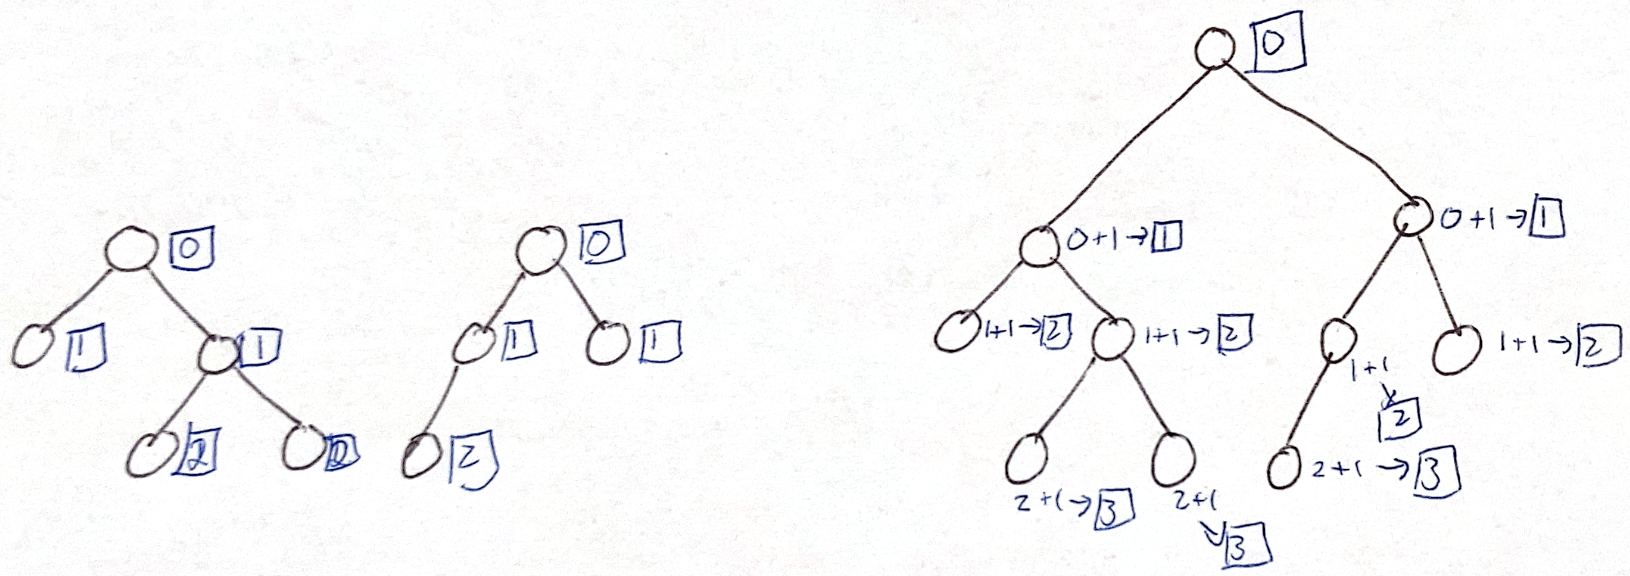
\includegraphics[width=4.5in]{add_root.png}
\end{center}
\end{frame}

\begin{frame} \frametitle{Optimal BST Step 2}
  For a chosen root index $r,$
  \[ e[i, j] = e[i, r-1] + e[r+1, j] + w(i, j) \]

  Optimize by choosing whichever root has minimal total cost:
  \[
    e[i, j] = 
        \begin{cases}
          q_{i-1} & \text{if } j=i-1 \\
          \min_{r \in [i:j]} (e[i, r-1] + e[r+1, j] + w(i, j)) & \text{if } i \leq j \\
        \end{cases} 
  \]
\end{frame}

\begin{frame} \frametitle{Optimal BST Step 3 -- core function}
  \begin{enumerate}
    \setcounter{enumi}{2}
    \item Design a divide-and-conquer algorithm that computes an \textbf{optimal value}.
    \stanza
  \end{enumerate}

  {\scriptsize
  \begin{algorithmic}[1]
    \Function{OBST-REC}{$p[1..n], q[0..n], i, j$}
    \If{ $j == (i-1)$ }
      \State \Return{ $q[i-1]$ }
    \EndIf
    \State $e = \infty$
    \For{$r$ from $i$ to $j$}
      \State $t = \text{OBST-REC}(p, q, i, r-1) + \text{OBST-REC}(p, q, r+1, j) + \text{W}(p, q, i, j)$
      \If{ $t < e$ }
        \State $e = t$
      \EndIf
    \EndFor
    \State \Return{ $e$ }
    \EndFunction
  \end{algorithmic}
  }
\end{frame}

\begin{frame} \frametitle{Optimal BST Step 3 -- helper functions}
  \begin{enumerate}
    \setcounter{enumi}{2}
    \item Design a divide-and-conquer algorithm that computes an \textbf{optimal value}.
    \stanza
  \end{enumerate}

  {\scriptsize
  \begin{algorithmic}[1]
    \Function{OBST-DC}{$p[1..n], q[0..n]$}
      \State \Return{ $\text{OBST-DC-REC}(p, q, 1, n)$ }
    \EndFunction
    \Function{W}{$p[1..n], q[0..n], i, j$}
      \State $w = 0$
      \For{$k$ from $i$ to $j$}
        \State $w = w + p[k]$
      \EndFor
      \For{$k$ from $i-1$ to $j$}
        \State $w = w + q[k]$
      \EndFor
      \State \Return{ $w$ }
    \EndFunction
  \end{algorithmic}
  }
\end{frame}

\begin{frame} \frametitle{Optimal BST Step 4.a}
  \begin{enumerate}
    \setcounter{enumi}{3}
    \item Design a dynamic programming algorithm that computes an \textbf{optimal value}.
    \begin{enumerate}
      \item \textbf{top-down} alternative: add table base case (\textbf{memoization})
      \stanza
    \end{enumerate}
\end{enumerate}

\begin{itemize}
  \item create hash table $T$
  \item use pair $(i, j)$ as key in table $T,$ storing $\text{OBST-REC}(p, q, i, j)$
\end{itemize}
\end{frame}

\begin{frame} \frametitle{Optimal BST Step 4.a -- helper functions}
  {\scriptsize
  \begin{algorithmic}[1]
    \Function{OBST-MEMOIZED}{$p[1..n], q[0..n]$}
      \State HASH-TABLE-CREATE($T$)
      \State \Return{ $\text{OBST-DC-REC}(p, q, T, 1, n)$ }
    \EndFunction
    \Function{W}{$p[1..n], q[0..n], i, j$}
      \State $w = 0$
      \For{$k$ from $i$ to $j$}
        \State $w = w + p[k]$
      \EndFor
      \For{$k$ from $i-1$ to $j$}
        \State $w = w + q[k]$
      \EndFor
      \State \Return{ $w$ }
    \EndFunction
  \end{algorithmic}
  }
\end{frame}

\begin{frame} \frametitle{Optimal BST Step 4.a -- core function}
  {\scriptsize
  \begin{algorithmic}[1]
    \Function{OBST-M}{$p[1..n], q[0..n], T, i, j$}
    \State $q = $ HASH-TABLE-SEARCH($T, (i, j)$)
    \If{ $q \ne$ NIL }
      \State \Return{ $q$ }
    \EndIf
    \If{ $j == (i-1)$ }
      \State \Return{ $q[i-1]$ }
    \EndIf
    \State $e = \infty$
    \For{$r$ from $i$ to $j$}
      \State $t = \text{OBST-M}(p, q, T, i, r-1) + \text{OBST-M}(p, q, T, r+1, j) + \text{W}(p, q, i, j)$
      \If{ $t < e$ }
        \State $e = t$
      \EndIf
    \EndFor
    \State $e.key = (i, j)$
    \State HASH-TABLE-INSERT($e$)
    \State \Return{ $e$ }
    \EndFunction
  \end{algorithmic}
  }
\end{frame}

\begin{frame} \frametitle{Optimal BST Step 4.b}
  \begin{enumerate}
    \setcounter{enumi}{3}
    \item Design a dynamic programming algorithm that computes an \textbf{optimal value}.
    \begin{enumerate}
      \item \textbf{top-down} alternative: add table base case (\textbf{memoization})
      \item \textbf{bottom-up} alternative: rewrite to use bottom-up loops instead of recursion
      \stanza
    \end{enumerate}
  \end{enumerate}
  \begin{itemize}
    \item create 2D array $e$ where $e[i][\, j] = \text{OBST-REC}(p, q, i, j)$
    \item \textbf{bottom-up:} write an explicit \textbf{for} loop that computes and stores every general case
  \end{itemize}
  \end{frame}
    
  \begin{frame} \frametitle{Optimal BST Step 4.b}
    {\footnotesize
    \begin{algorithmic}[1]
      \Function{OBST-BU}{$p[1..n], q[0..n]$}
      \State Create array $e[1..n+1][0..n]$ \Comment{unusual index range}
      \For{$i$ from 1 to $n+1$}
        \State $e[i][i-1] = q[i-1]$ \Comment{ base cases }
      \EndFor
      \For{$\ell$ from 1 to $n$}
        \For{$i$ from 1 to $n-\ell+1$}
          \State $j = i + \ell - 1$
          \State $e[i][j] = \infty$
          \For{$r = i$ to $j$}
            \State $t = e[i][r-1] + e[r+1][j] + W(p, q, i, j)$
            \If{ $t < e[i][j]$}
              \State $e[i][j] = t$
            \EndIf
          \EndFor
        \EndFor
      \EndFor
      \State \Return $e[1][n]$
      \EndFunction
    \end{algorithmic}
    }
\end{frame}
  
\begin{frame} \frametitle{Optimal BST Bottom-Up Analysis}
  \begin{itemize}
    \item Create array $e$: $\Theta(n^2)$
    \item Base cases: $\Theta(n)$
    \item General cases:
      \begin{itemize}
        \item \textbf{for} loop over $\ell$: $\Theta(n)$ iterations
        \item nested \textbf{for} loop over $i$: $\Theta(n)$ iterations
        \item nested \textbf{for} loop over $r$: $\Theta(n)$ iterations
        \item call $W(p, q, i, j)$: $\Theta(n)$ time
      \end{itemize}
    \item total $\Theta(n^4)$ time
    \item bottleneck is calls to $W$
    \item can precompute and cache $W$ values in their own table
  \end{itemize}
\end{frame}

\begin{frame} \frametitle{Optimal BST Final Draft}
  {\tiny
  \begin{algorithmic}[1]
    \Function{OBST-BU}{$p[1..n], q[0..n]$}
    \State Create array $e[1..n+1][0..n]$ \Comment{unusual index range}
    \State Create array $w[1..n+1][0..n]$ \Comment{$w[i][j] = W(p, q, i, j)$}
    \For{$i$ from 1 to $n+1$}
      \State $e[i][i-1] = q[i-1]$ \Comment{ base cases }
      \State $w[i][i-1] = q[i-1]$
    \EndFor
    \For{$\ell$ from 1 to $n$}
      \For{$i$ from 1 to $n-\ell+1$}
        \State $j = i + \ell - 1$
        \State $e[i][j] = \infty$
        \State $w[i][j] = w[i][j-1] + p[j] + q[j]$
        \For{$r = i$ to $j$}
          \State $t = e[i][r-1] + e[r+1][j] + w[i][j]$
          \If{ $t < e[i][j]$}
            \State $e[i][j] = t$
          \EndIf
        \EndFor
      \EndFor
    \EndFor
    \State \Return $e[1][n]$
    \EndFunction
  \end{algorithmic}
  }
\end{frame}

\begin{frame} \frametitle{Optimal BST Final Draft Analysis}
  \begin{itemize}
    \item three nested loop
    \item body of innermost loop is now only $\Theta(1)$
    \item $\text{OBST-BU}$ takes $\Theta(n^3)$ time
  \end{itemize}
\end{frame}

\end{document}
